\documentclass[11pt,a4paper]{article}
\usepackage[utf8]{inputenc}
\usepackage[margin=1in]{geometry}
\usepackage{graphicx}
\usepackage{amsmath}
\usepackage{titlesec}
\usepackage{titling}
\usepackage{caption}
\usepackage{tikz}
\usetikzlibrary{shapes.geometric, arrows, positioning}
\usepackage{booktabs}
\usepackage{cite}
\usepackage{hyperref}

\titleformat{\section}{\large\bfseries}{\thesection}{1em}{}
\titlespacing*{\section}{0pt}{1.2ex plus 1ex minus .2ex}{0.5ex plus .2ex}

\begin{document}

\begin{center}
    % \includegraphics[width=2.5cm]{iitkgp_logo.png} % Add logo here
    
    {\Large \bfseries Indian Institute of Technology Kharagpur}\\[0.2cm]
    {\large Department of Industrial and Systems Engineering}\\[0.2cm]
    {\normalsize BTP-I Mid-Semester Project Summary}\\[0.1cm]
    {\normalsize Autumn Semester 2026--27}\\[0.3cm]
    \rule{\textwidth}{0.5pt}
\end{center}

\noindent
\textbf{Name:} \makebox[4cm][l]{[Your Name]} 
\textbf{Roll No.:} \makebox[3cm][l]{[Your Roll No.]} 
\textbf{Supervisor:} Prof. Sarada Prasad Sarmah

\vspace{0.4cm}
\begin{center}
    {\Large \bfseries Advanced Pharmacovigilance: A Multi-Gate Polypharmacy Mining Framework Using Disproportionality Analysis and Machine Learning}
\end{center}
\vspace{0.2cm}

\section*{Background and Motivation}
Adverse Drug Reactions (ADRs) are a leading cause of morbidity and mortality globally. With the increasing prevalence of polypharmacy (the concurrent use of multiple medications), identifying harmful drug-drug interactions is critical. Spontaneous reporting systems, such as the FDA Adverse Event Reporting System (FAERS), collect millions of post-marketing safety reports. However, analyzing this data is highly challenging due to extreme sparsity, reporting biases, and the combinatorial explosion of potential multi-drug interactions.

While conventional data mining in pharmacovigilance focuses primarily on single-drug effects or 2-drug interactions, clinically significant ADRs are often triggered by higher-order combinations (3 or more drugs). Identifying these signals requires differentiating the true synergistic interaction from the individual toxicities of the constituent drugs. This project aims to address this gap by developing a robust, mathematically defensible pipeline that goes beyond mere co-occurrence, rigorously isolating authentic 3-drug polypharmacy signals from millions of nested FAERS records.

\section*{Related Work and Research Direction}
Prior research extensively explores 2-drug interactions in pharmacovigilance. Ibrahim et al. (2016) proposed a Hybrid Apriori approach that pairs frequent itemset mining with the Proportional Reporting Ratio (PRR) and Chi-square statistics to detect Drug Interaction Adverse Event (DIAE) signals. Crucially, they employed a Logistic Regression model to test for confounding and to isolate the specific 2-drug interaction coefficient [1].

However, scaling these methodologies to 3-drug combinations introduces significant statistical noise and computational complexity. Simple rule mining generates thousands of spurious patterns driven by highly reported baseline drugs. This project extends the methodology of Ibrahim et al. by introducing a "Multi-Gate" statistical framework for 3-drug combinations, utilizing FP-Growth for efficient candidate generation, Hierarchical Reporting Odds Ratio (ROR) comparisons, and 3-way Logistic Regression with Benjamini-Hochberg False Discovery Rate (FDR) correction to rigorously control type I errors.

\section*{Aim and Objectives}
The primary aim of this project is to develop and evaluate a scalable, automated pipeline to detect and statistically validate 3-drug polypharmacy adverse event signals from the OpenFDA database. The specific objectives are:
\begin{itemize}
    \item \textbf{Data Integration:} To engineer a pipeline capable of parsing millions of nested OpenFDA JSON reports into a high-performance relational database (DuckDB).
    \item \textbf{Candidate Generation:} To apply the FP-Growth algorithm to efficiently mine frequent 3-drug itemsets that meet minimum absolute and relative support thresholds.
    \item \textbf{Hierarchical Validation:} To compute the ROR for 3-drug combinations and mathematically compare them against all lower-order components (individual drugs and pairs) to ensure the triplet exhibits unique interaction risk.
    \item \textbf{Statistical Modeling:} To implement a 3-way Logistic Regression model, extracting the interaction coefficient while adjusting for multiple testing using FDR correction.
    \item \textbf{Predictive Analytics:} To evaluate the performance of advanced Machine Learning models (XGBoost, Random Forest, Lasso) in predicting the occurrence of severe ADRs based on patient drug exposure profiles.
\end{itemize}

\section*{Proposed System Architecture}
The system architecture separates data ingestion, statistical gating, predictive modeling, and interactive visualization into modular components.

\begin{center}
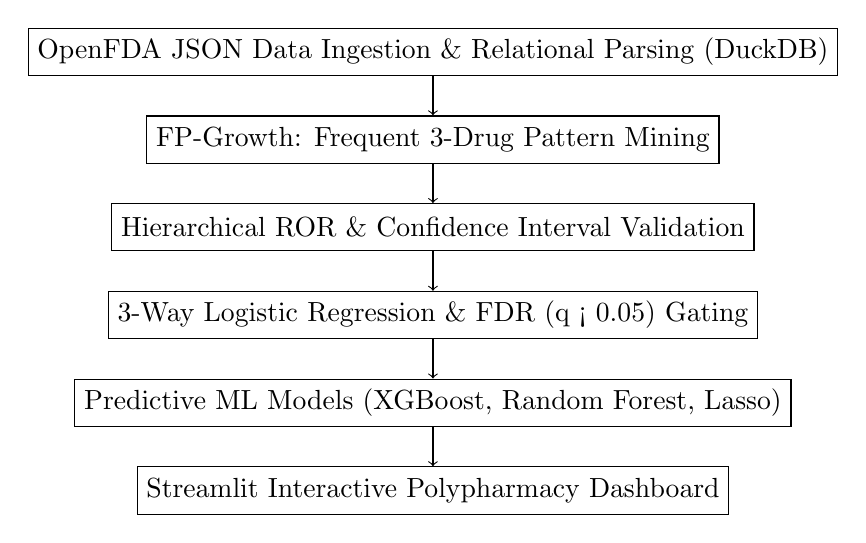
\begin{tikzpicture}[node distance=1.2cm, auto,
    box/.style={rectangle, draw, align=center, minimum width=6cm, minimum height=0.6cm}]
    
    \node[box] (data) {OpenFDA JSON Data Ingestion \& Relational Parsing (DuckDB)};
    \node[box, below=0.5cm of data] (fp) {FP-Growth: Frequent 3-Drug Pattern Mining};
    \node[box, below=0.5cm of fp] (ror) {Hierarchical ROR \& Confidence Interval Validation};
    \node[box, below=0.5cm of ror] (lr) {3-Way Logistic Regression \& FDR (q < 0.05) Gating};
    \node[box, below=0.5cm of lr] (ml) {Predictive ML Models (XGBoost, Random Forest, Lasso)};
    \node[box, below=0.5cm of ml] (dash) {Streamlit Interactive Polypharmacy Dashboard};
    
    \draw[->] (data) -- (fp);
    \draw[->] (fp) -- (ror);
    \draw[->] (ror) -- (lr);
    \draw[->] (lr) -- (ml);
    \draw[->] (ml) -- (dash);
    
\end{tikzpicture}
\end{center}

\section*{Current Progress}
A functional prototype of the end-to-end framework has been implemented and validated on a subset of the 2023 FAERS dataset. The current achievements include:
\begin{itemize}
    \item \textbf{Ingestion Pipeline:} Developed an automated script that securely fetches, streams, and flattens OpenFDA zip partitions directly into a DuckDB analytical database without intermediary disk extraction, dramatically optimizing storage and ingestion speed.
    \item \textbf{Multi-Gate Polypharmacy Miner:} Implemented the core analytical engine in Python using \texttt{mlxtend} and \texttt{statsmodels}. The engine successfully mines 3-drug combinations, computes subset ROR comparisons (producing a novel \textit{Interaction Strength} metric), and fits the 3-way Logistic Regression model.
    \item \textbf{Signal Detection:} The pipeline successfully detected true, statistically significant polypharmacy signals (e.g., Fentanyl + Opana + Percocet leading to Overdose) that survived all mathematical gating and FDR thresholds.
    \item \textbf{Advanced ML Models:} Designed an automated module that engineers sparse one-hot encoded drug matrices and trains XGBoost, Random Forest, and Lasso Regression models to classify adverse event occurrences, capturing complex non-linear drug interactions.
    \item \textbf{Interactive Dashboard:} Built a multi-page Streamlit application that dynamically visualizes the surviving polypharmacy signals, predictive model metrics (Accuracy, ROC-AUC, F1), and provides an exploratory interface for single-drug ADR statistics.
\end{itemize}

\section*{Planned Experimental Study and Further Development}
The next phase of the project will focus on scaling the framework and incorporating temporal analysis:
\begin{itemize}
    \item \textbf{Full-Scale Execution:} Execute the ingestion and Multi-Gate mining pipeline over the entire multi-year OpenFDA database (millions of reports) to uncover hidden, rare 3-drug signals.
    \item \textbf{Temporal Persistence Analysis:} Analyze quarter-over-quarter growth rates of detected signals to ensure they are consistent over time rather than isolated anomalies, culminating in a robust \textit{Emerging Signal Score}.
    \item \textbf{Model Optimization \& Deep Learning:} Tune the hyperparameters of the XGBoost and Random Forest classifiers. Explore the application of tabular transformer architectures (e.g., TabNet) if computational resources permit.
    \item \textbf{FDA Label Integration:} Integrate the openFDA Drug Labeling API to automatically cross-reference discovered signals against documented manufacturer warnings.
\end{itemize}

\section*{Expected Outcome}
This project is expected to deliver a highly defensible, end-to-end data mining and machine learning framework capable of separating true multi-drug interaction signals from baseline reporting noise in massive pharmacovigilance datasets. The resulting open-source pipeline and interactive dashboard will serve as a powerful exploratory tool, demonstrating a rigorous statistical methodology that improves upon conventional 2-drug association rule mining.

\vspace{0.3cm}
\section*{References}
\begin{enumerate}
    \item[1] H. Ibrahim, A. El-Makky, and G. Taha, ``Mining association patterns of drug-interactions using post marketing FDA's spontaneous reporting data,'' \textit{Journal of Biomedical Informatics}, 2016.
\end{enumerate}

\vspace{1.5cm}
\noindent
\begin{tabular}{@{}p{0.5\linewidth} p{0.5\linewidth}@{}}
\textbf{Submitted by} & \textbf{Supervisor's Signature} \\[1.5cm]
\rule{6cm}{0.4pt} & \rule{6cm}{0.4pt} \\
\makebox[6cm][l]{[Your Name]} & \makebox[6cm][l]{Prof. Sarada Prasad Sarmah} \\
\makebox[6cm][l]{Roll No.: [Your Roll No.]} & \makebox[6cm][l]{Department of Industrial and Systems Engineering} \\
\makebox[6cm][l]{Department of Industrial and Systems Engineering} & \makebox[6cm][l]{IIT Kharagpur} \\
\makebox[6cm][l]{IIT Kharagpur} & \\
\end{tabular}

\end{document}
